% This is a LaTeX thesis template for Adam Mickiewicz University.
% to be used with Rmarkdown
% This template was produced by Jakub Nowosad
% Version: 16 February 2020

% Inspired by:
% This is a LaTeX thesis template for Monash University.
% to be used with Rmarkdown
% This template was produced by Rob Hyndman
% Version: 6 September 2016

\documentclass{amuthesis}
%\usepackage[polish]{babel}
%\usepackage{polski}
%\renewcommand{\figurename}{Figure} % Redefine default figure caption %
%\renewcommand{\tablename}{Table} % Redefine default table caption %
%%%%%%%%%%%%%%%%%%%%%%%%%%%%%%%%%%%%%%%%%%%%%%%%%%%%%%%%%%%%%%%
% Add any LaTeX packages and other preamble here if required
%%%%%%%%%%%%%%%%%%%%%%%%%%%%%%%%%%%%%%%%%%%%%%%%%%%%%%%%%%%%%%%
\usepackage{booktabs,tabularx} % Allows kableExtra to work %
\usepackage{indentfirst} % Adds indent in the first paragraph %
\usepackage{bookmark} % Adds indent in the first paragraph %
\usepackage{booktabs}
\usepackage{longtable}
\usepackage{array}
\usepackage{multirow}
\usepackage{wrapfig}
\usepackage{float}
\usepackage{colortbl}
\usepackage{pdflscape}
\usepackage{tabu}
\usepackage{threeparttable}
\usepackage{threeparttablex}
\usepackage[normalem]{ulem}
\usepackage{makecell}
\usepackage{xcolor}

\author{Tomasz Matuszek}
\title{Measuring an impact of the Landsat 8 thermal band on the
supervised land cover classification results}
\def\titleeng{Ocena wpływu zastosowania kanału termalnego Landsat na
wyniki nadzorowanej klasyfikacji pokrycia terenu}
\def\degreetitle{Engineer's thesis}
\def\major{Geoinformation}
\def\albumid{455828}
\def\thesisyear{2023}
% Add subject and keywords below
\hypersetup{
     %pdfsubject={The Subject},
     %pdfkeywords={Some Keywords},
     pdfauthor={Tomasz Matuszek},
     pdftitle={Measuring an impact of the Landsat 8 thermal band on the
supervised land cover classification results},
     pdfproducer={quarto with LaTeX}
}

\bibliography{thesis,packages}

\begin{document}

\pagenumbering{arabic}

\titlepage

\bookmarksetup{startatroot}

\hypertarget{abstract}{%
\chapter*{Abstract}\label{abstract}}
\addcontentsline{toc}{chapter}{Abstract}

\markboth{Abstract}{Abstract}

\textbf{Abstrakt}

Streszczenie powinno przedstawiać skrótowo główny problem pracy i jego
rozwiązanie. Możliwa struktura streszczenia to: (1) 1-3 zdania wstępu do
problemu (czym się zajmujemy, dlaczego jest to ważne, jakie są
problemy/luki do wypełnienia), (2) 1 zdanie opisujące cel pracy, (3) 1-3
zdania przedstawiające użyte materiały (dane) i metody (techniki,
narzędzia), (4) 1-3 zdania obrazujące główne wyniki pracy, (5) 1-2
zdania podsumowujące; możliwe jest też określenie dalszych
kroków/planów.

Słowa kluczowe: (4-6 słów/zwrotów opisujących treść pracy, które nie
wystąpiły w tytule)

\textbf{Abstract}

The abstract must be consistent with the above text.

Keywords: (as stated before)

\newpage

\setstretch{1.2}\sf\tighttoc\doublespacing

\bookmarksetup{startatroot}

\hypertarget{sec-intro}{%
\chapter{Introduction}\label{sec-intro}}

\begin{itemize}
\item
  applications and relevance of land cover maps
\item
  machine learning and supervised classification of satellite images as
  a tool for creating land cover maps
\item
  pointing out that thermal band if often omitted in land cover
  classification models, exact impact of thermal factor isn't fully
  clear
\item
  goal of the thesis is to create land cover map of Poznań metropolitan
  area and measure the impact of thermal band on the model results
\end{itemize}

\begin{center}\rule{0.5\linewidth}{0.5pt}\end{center}

Wprowadzenie powinno mieć charakter opisu od ogółu do szczegółu (np.
trzy-pięć paragrafów). Pierwszy paragraf powinien być najbardziej
ogólny, a kolejne powinny przybliżać czytelnika do problemu.
Przedostatni paragraf powinien określić jaki jest problem (są problemy),
który praca ma rozwiązać i dlaczego jest to (są one) ważne.

Wprowadzenie powinno być zakończone stwierdzeniem celu pracy. Dodatkowo
tutaj może znaleźć się również krótki opis co zostało zrealizowane w
pracy.

Pisząc ten rozdział proszę pomyśleć o osobach, które zupełnie nie znają
opisywanej tematyki. Należy tutaj krok po kroku wyjaśnić podstawowe
koncepcje, istotność problemu, wyniki poprzednich podobnych badań, itd.
Ten rozdział obejmuje tylko kwestie, które już zostały wykonane przez
inne osoby - nowe wyniki mają swoje miejsce w rozdziale
\textbf{?@sec-wyniki}.

Każda kwestia opisana w tym rozdziale powinna być cytowana. Dodatnie
cytowania odbywa się poprzez uzupełnienie pliku \texttt{thesis.bib}
zapisem w formacie BibTeX, a następnie dodanie nazwy referencji
poprzedzonej znakiem \texttt{@}. Przykładowo, zacytowanie książki
Geocomputation with R odbywa się poprzez
\autocite{lovelace_geocomputation_2019}.

W przypadku, gdy cytowanie zostało poprawnie wpisane oraz istnieje w
pliku \texttt{thesis.bib} to bibliografia powinna się automatycznie
wygenerować na końcu pracy.

W przypadku, gdy praca dyplomowa opisuje konkretny obszar to można po
tym rozdziale stworzyć kolejny rozdział opisujący ``obszar badań''.

Ten i kolejne rozdziału moją mieć także podrozdziały. Tworzenie
podrozdziałów polega na stworzeniu nowej linii rozpoczynającej się od
znaków \texttt{\#\#} a następnie tytułu podrozdziału. Dodatkowo w
postaci \texttt{\{\#sec-\}} można dodać skrót nazwy
rozdziału/podrozdziału umożliwiający odnoszenie się do niego używając
operatora \texttt{{[}-@sec{]}}.

\bookmarksetup{startatroot}

\hypertarget{sec-data-methods}{%
\chapter{Materials and methods}\label{sec-data-methods}}

Workflow of the study consisted of several stages: preprocessing of
source data (described in Sections \ref{sec-sat} and
\ref{sec-landcover}), creating training dataset, model's parameters
tuning, land cover map prediction, model quality assessment and
evaluating the impact of thermal band on the model's results (Figure
\ref{fig-rycina4}). Each of these steps was performed using R
programming language \autocite{R-base}. Final visualisations were
created in QGIS software \autocite{qgis_development_team_qgis_2009}.
Both programming environment and GIS software used in this process are
open-source.

\begin{figure}

{\centering 

\begin{figure}[H]

{\centering 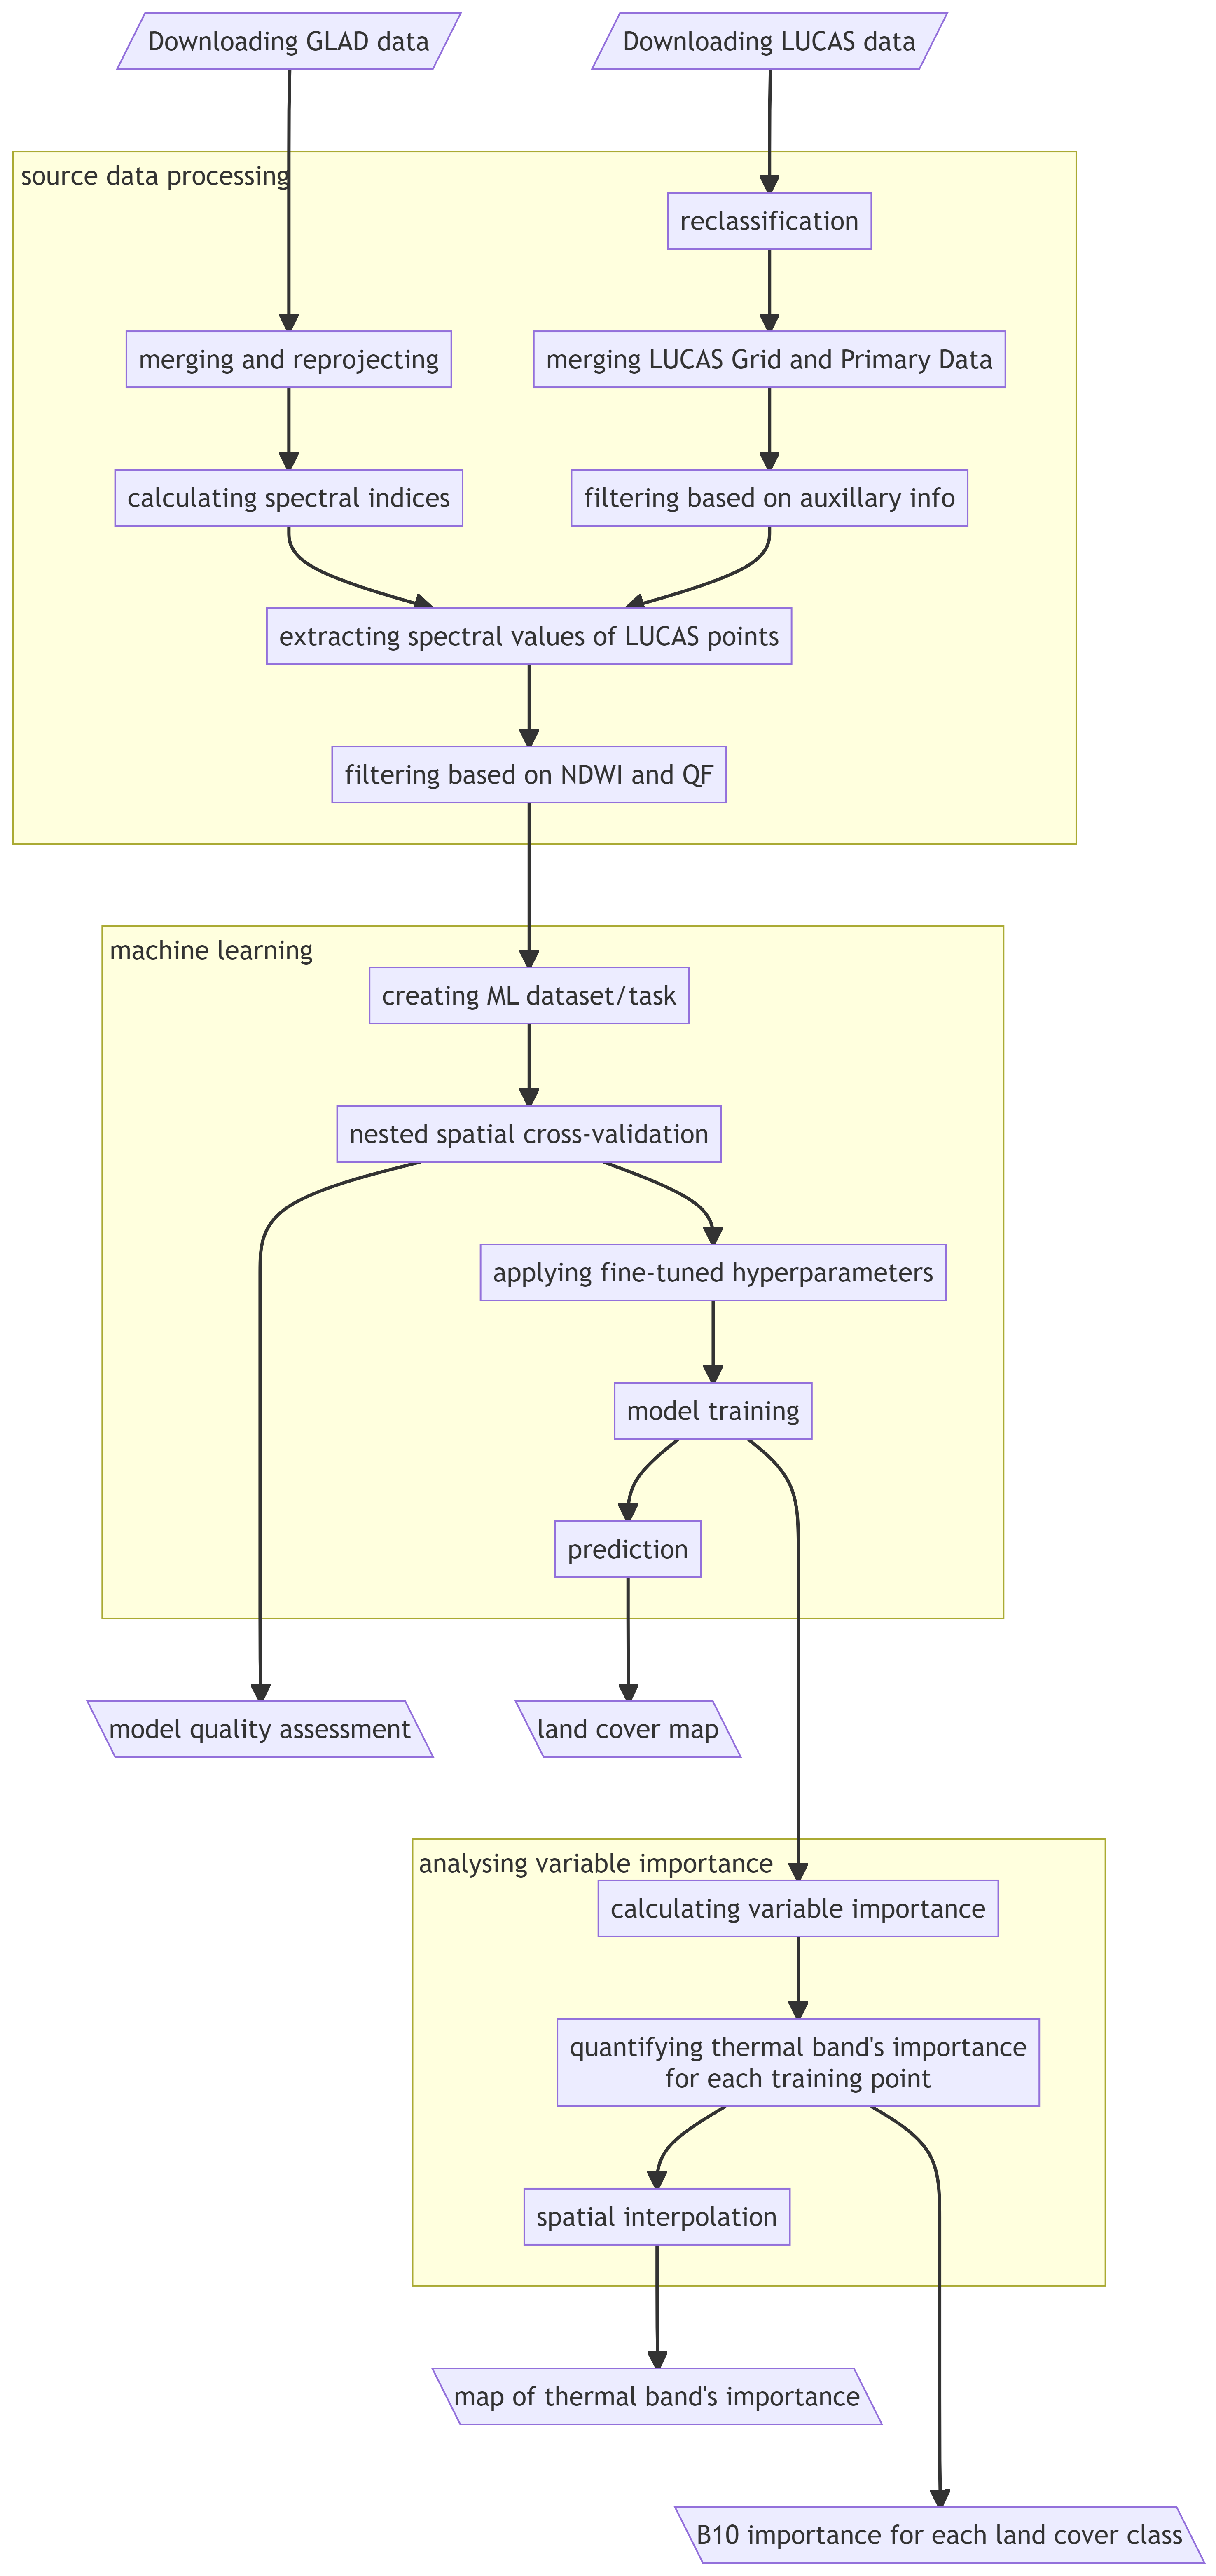
\includegraphics[width=4in,height=8.26in]{./02-roz2_files/figure-latex/mermaid-figure-1.png}

}

\end{figure}

}

\caption{\label{fig-rycina4}General workflow of the study}

\end{figure}

Landsat ARD dataset, provided by GLAD laboratory at the Univeristy of
Maryland, was used as a source of multi-spectral satellite imagery.
Training points were obtained from LUCAS dataset created by Eurostat
\autocite{dandrimont_harmonised_2020}. Both data sets were downloaded
for central-western part of Poland which was chosen as training area
(Figure \ref{fig-rycina1}). This data was pre-processed and then used to
train the model and validate its performance.

\begin{figure}[t]

{\centering 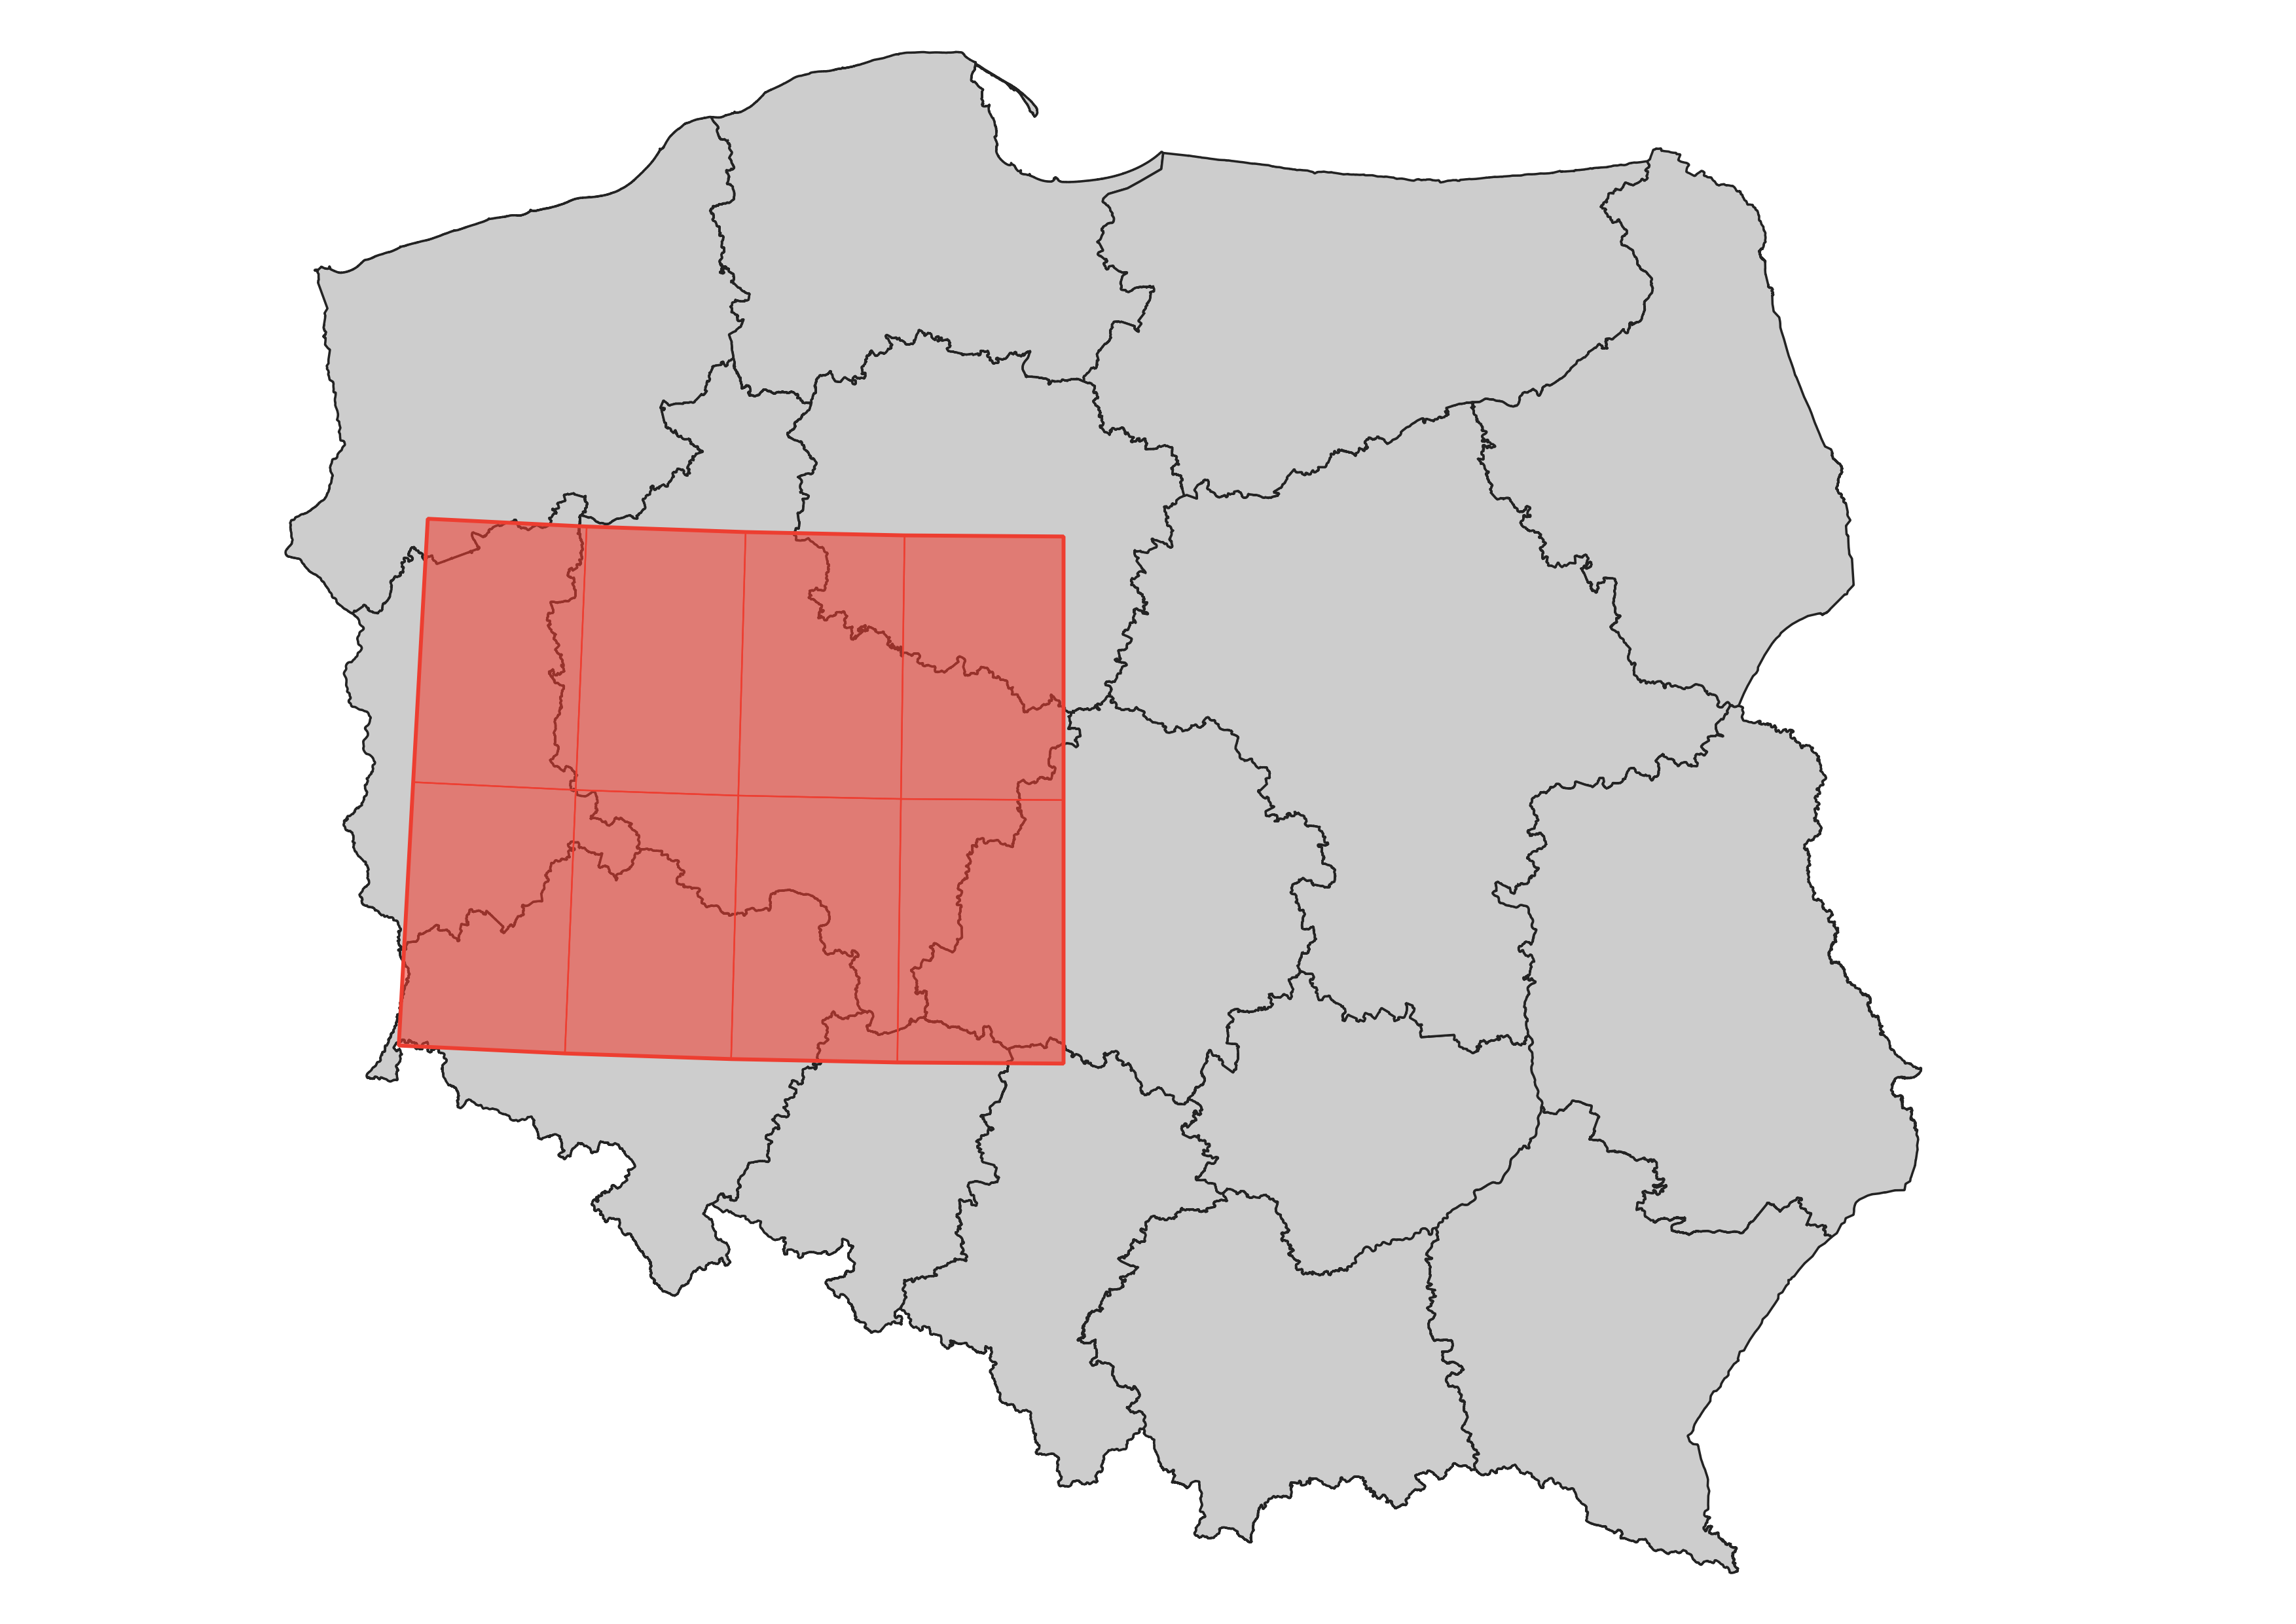
\includegraphics[width=1\textwidth,height=4.16667in]{./figures/study_area.png}

}

\caption{\label{fig-rycina1}Training area}

\end{figure}

\hypertarget{sec-sat}{%
\section{Satellite imagery}\label{sec-sat}}

Satellite imagery from GLAD Landsat ARD is available in 16-day interval
composites and is divided into 1° x 1° tiles. Processing of original
Landsat images performed by GLAD team included converting spectral bands
to top-of-atmosphere (TOA) reflectance, converting thermal band to
brightness temperature (BT) in Kelvins, scaling the values of all bands
as well as adding quality flag for every pixel
\autocite{potapov_landsat_2020}.

Satellite images for eight 1° x 1° tiles, covering the study area
(Figure \ref{fig-rycina1}), were downloaded using GLAD Tools v1.1 and
PERL programming language. These images are from 10th interval of the
year 2018, so downloaded mosaics consist of images created between
24.05.2018 and 8.06.2018. All downloaded images were merged and
reprojected from WGS84 coordinate reference system (EPSG:4326) to UTM
zone 33N (EPSG:32633). Every band was also resampled from 0.00025°
resolution (corresponding to 27.83 m on equator) to 30 meters
resolution.

In addition, four spectral indices were derived: Normalized Difference
Vegetation Index (NDVI), Modified Normalized Difference Water Index
(MNDWI), Normalized Difference Moisture Index (NDMI) and Modified Bare
soil Index (MBI). Formulas used to calculate these indices can be found
in Table \ref{tbl-tabela1}.

\hypertarget{tbl-tabela1}{}
\begin{table}
\caption{\label{tbl-tabela1}Formulas of spectral indices dervied from Landsat data }\tabularnewline

\centering
\begin{tabular}{|>{\raggedright\arraybackslash}p{4cm}|>{}l|>{}l|}
\toprule
\textbf{band/index} & \textbf{abbreviation} & \textbf{formula}\\
\midrule
Blue & B2 & -\\
\hline
Green & B3 & -\\
\hline
Red & B4 & -\\
\hline
Near Infrared & B5 (NIR) & -\\
\hline
Short-wave Infrared 1 & B6 (SWIR1) & -\\
\hline
Short-wave Infrared 2 & B7 (SWIR2) & -\\
\hline
Thermal & B10 (TIRS1) & -\\
\hline
Normalized Difference Vegetation Index & NDVI & (B5 -B4) / (B4 + B5)\\
\hline
Modified Normalized Difference Water Index & MNDWI & (B3 - B6) / (B3 + B6)\\
\hline
Normalized Difference Moisture Index & NDMI & (B5 - B6) / (B5 + B6)\\
\hline
Modified Bare Surface Index & MBI & (B6 - B7 - B5) / (B6 + B7 + B5) + 0.5\\
\bottomrule
\end{tabular}
\end{table}

\hypertarget{sec-landcover}{%
\section{Land cover data}\label{sec-landcover}}

Data collected during LUCAS survey performed by Eurostat was chosen as
land cover training set. At the moment of writing, it is the most
accurate and comprehensive dataset containing information about land use
and land cover \autocite{pflugmacher_mapping_2019} due to the fact, that
every point was either manually photo-interpreted or assessed during
\emph{in-situ} visit.

LUCAS survey consists of two phases. First phase is based on grid of
points with 2km spacing covering whole territory of the European Union
(which equals to more than 1 million points). Each point of the grid is
visually interpreted using ortho-photos or satellite images, and
classified into one of seven major land-cover classes. These classes
are: arable land, permanent crops, grassland, wooded areas/shrub land,
bare land, artificial land and water. In the second phase, a subsample
of grid points is selected and then visited by Eurostat surveyors. They
classify each point according to full LUCAS land cover and land use
classification. The survey takes place in the spring and summer in order
to observe chosen places in high vegetation season
\autocite{dandrimont_harmonised_2020}.

Surveyor not only assign land cover and land use classes to points, but
they also add auxillary information such as plant species present at the
site, percentage of land coverage for a chosen class, height of the
trees and their maturity, as well as information about water management
and irrigation. If there are more than one land cover/land use types at
the point, observer can also assign a secondary class for every LUCAS
point.

Majority of the training points used for the classification model were
points from the second phase of LUCAS survey, also called LUCAS Primary
Data. I downloaded a total of 4,153 points for the study area.
Pre-processing step included omitting records with missing data,
excluding artificial linear land cover classes (e.g.~roads or railways)
and excluding points that were surveyed more than 500 meters from their
theoretical location. In the next step, detailed land cover classes were
aggregated into eight main groups of land cover types. Two of them -
grassland and shrubland were additionally aggregated into one land cover
class. Then, I filtered some of the classes according to the percentage
of land coverage or percentage of impervious surface coverage (Table
\ref{tbl-tabela2}).

\hypertarget{tbl-tabela2}{}
\begin{table}
\caption{\label{tbl-tabela2}Filters applied to reclassified land cover groups. IMP - impervious
surface, HRB - herbaceous plants cover, TC - tree cover }\tabularnewline

\centering
\begin{tabular}{|>{}l|>{}l|>{}l|>{\raggedright\arraybackslash}p{4cm}|>{\raggedright\arraybackslash}p{2cm}|}
\toprule
\textbf{ID} & \textbf{LC class} & \textbf{LUCAS Grid} & \textbf{LUCAS Primary Data} & \textbf{Filters}\\
\midrule
\cellcolor[HTML]{e8ef5f}{\textbf{1}} & arable land & - & B00 (Cropland) & <30\% IMP\\
\hline
\cellcolor[HTML]{80dc59}{\textbf{2}} & grasslands & - & E00 (Grassland), D00 (Shrubland) & >50\% HRB; <30\% IMP\\
\hline
\cellcolor[HTML]{11a723}{\textbf{3}} & forests & - & C00 (Woodland) & >50\% TC; <20\% IMP\\
\hline
\cellcolor[HTML]{b7b7b7}{\textbf{4}} & bare land & 6 (Bare surface) & F00 (Bare land) & -\\
\hline
\cellcolor[HTML]{ea001f}{\textbf{5}} & artificial land & 7 (Artificial areas) & A00 (Artificial land) & >70\% IMP\\
\hline
\cellcolor[HTML]{56a4f3}{\textbf{6}} & water bodies & 8 (Inland water) & G00 (Water areas) & -\\
\hline
\cellcolor[HTML]{7a338c}{\textbf{7}} & wetlands & - & H00 (Wetlands) & -\\
\bottomrule
\end{tabular}
\end{table}

For the least frequent classes in the LUCAS Primary Data dataset - bare
land, artificial land and water bodies - I also added points classified
during the first phase of LUCAS survey (Figure \ref{fig-rycina2}). This
step was necessary to ensure that every land cover class is represented
by enough number of points. It was not possible only for wetlands class,
because of lack of such category in the first phase classification. At
the end of the pre-processing, dataset was left with 3,778 training
points \autocite{oliver_buck_analysis_2015}.

\begin{figure}[t]

{\centering 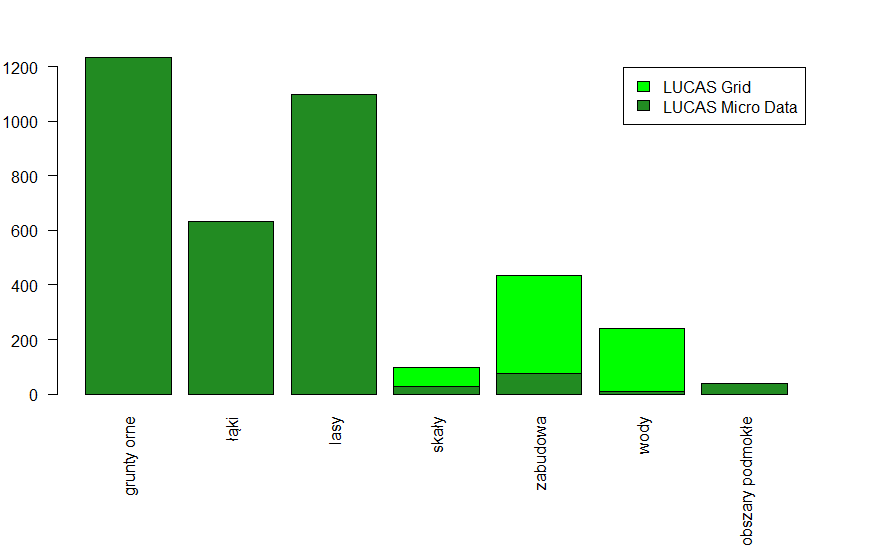
\includegraphics[width=1\textwidth,height=3.64583in]{./figures/lucas_data.png}

}

\caption{\label{fig-rycina2}Distribution of points by land cover class
after pre-processing}

\end{figure}

After extracting values from Landsat ARD raster, LUCAS points were also
filtered using quality flag provided. Only points with clear-sky quality
flag were taken into account during the process of model training.
Moreover, water bodies points in which NDWI was lower than 0 were also
excluded. These two conditions eliminated over 400 points in total.

Training set obtained after pre-processing can be seen in Figure
\ref{fig-rycina3}. Spatial distribution of data points was fairly even
and due to the structure of LUCAS data set, every point was located at
least 2 kilometers from another one.

\begin{figure}[t]

{\centering 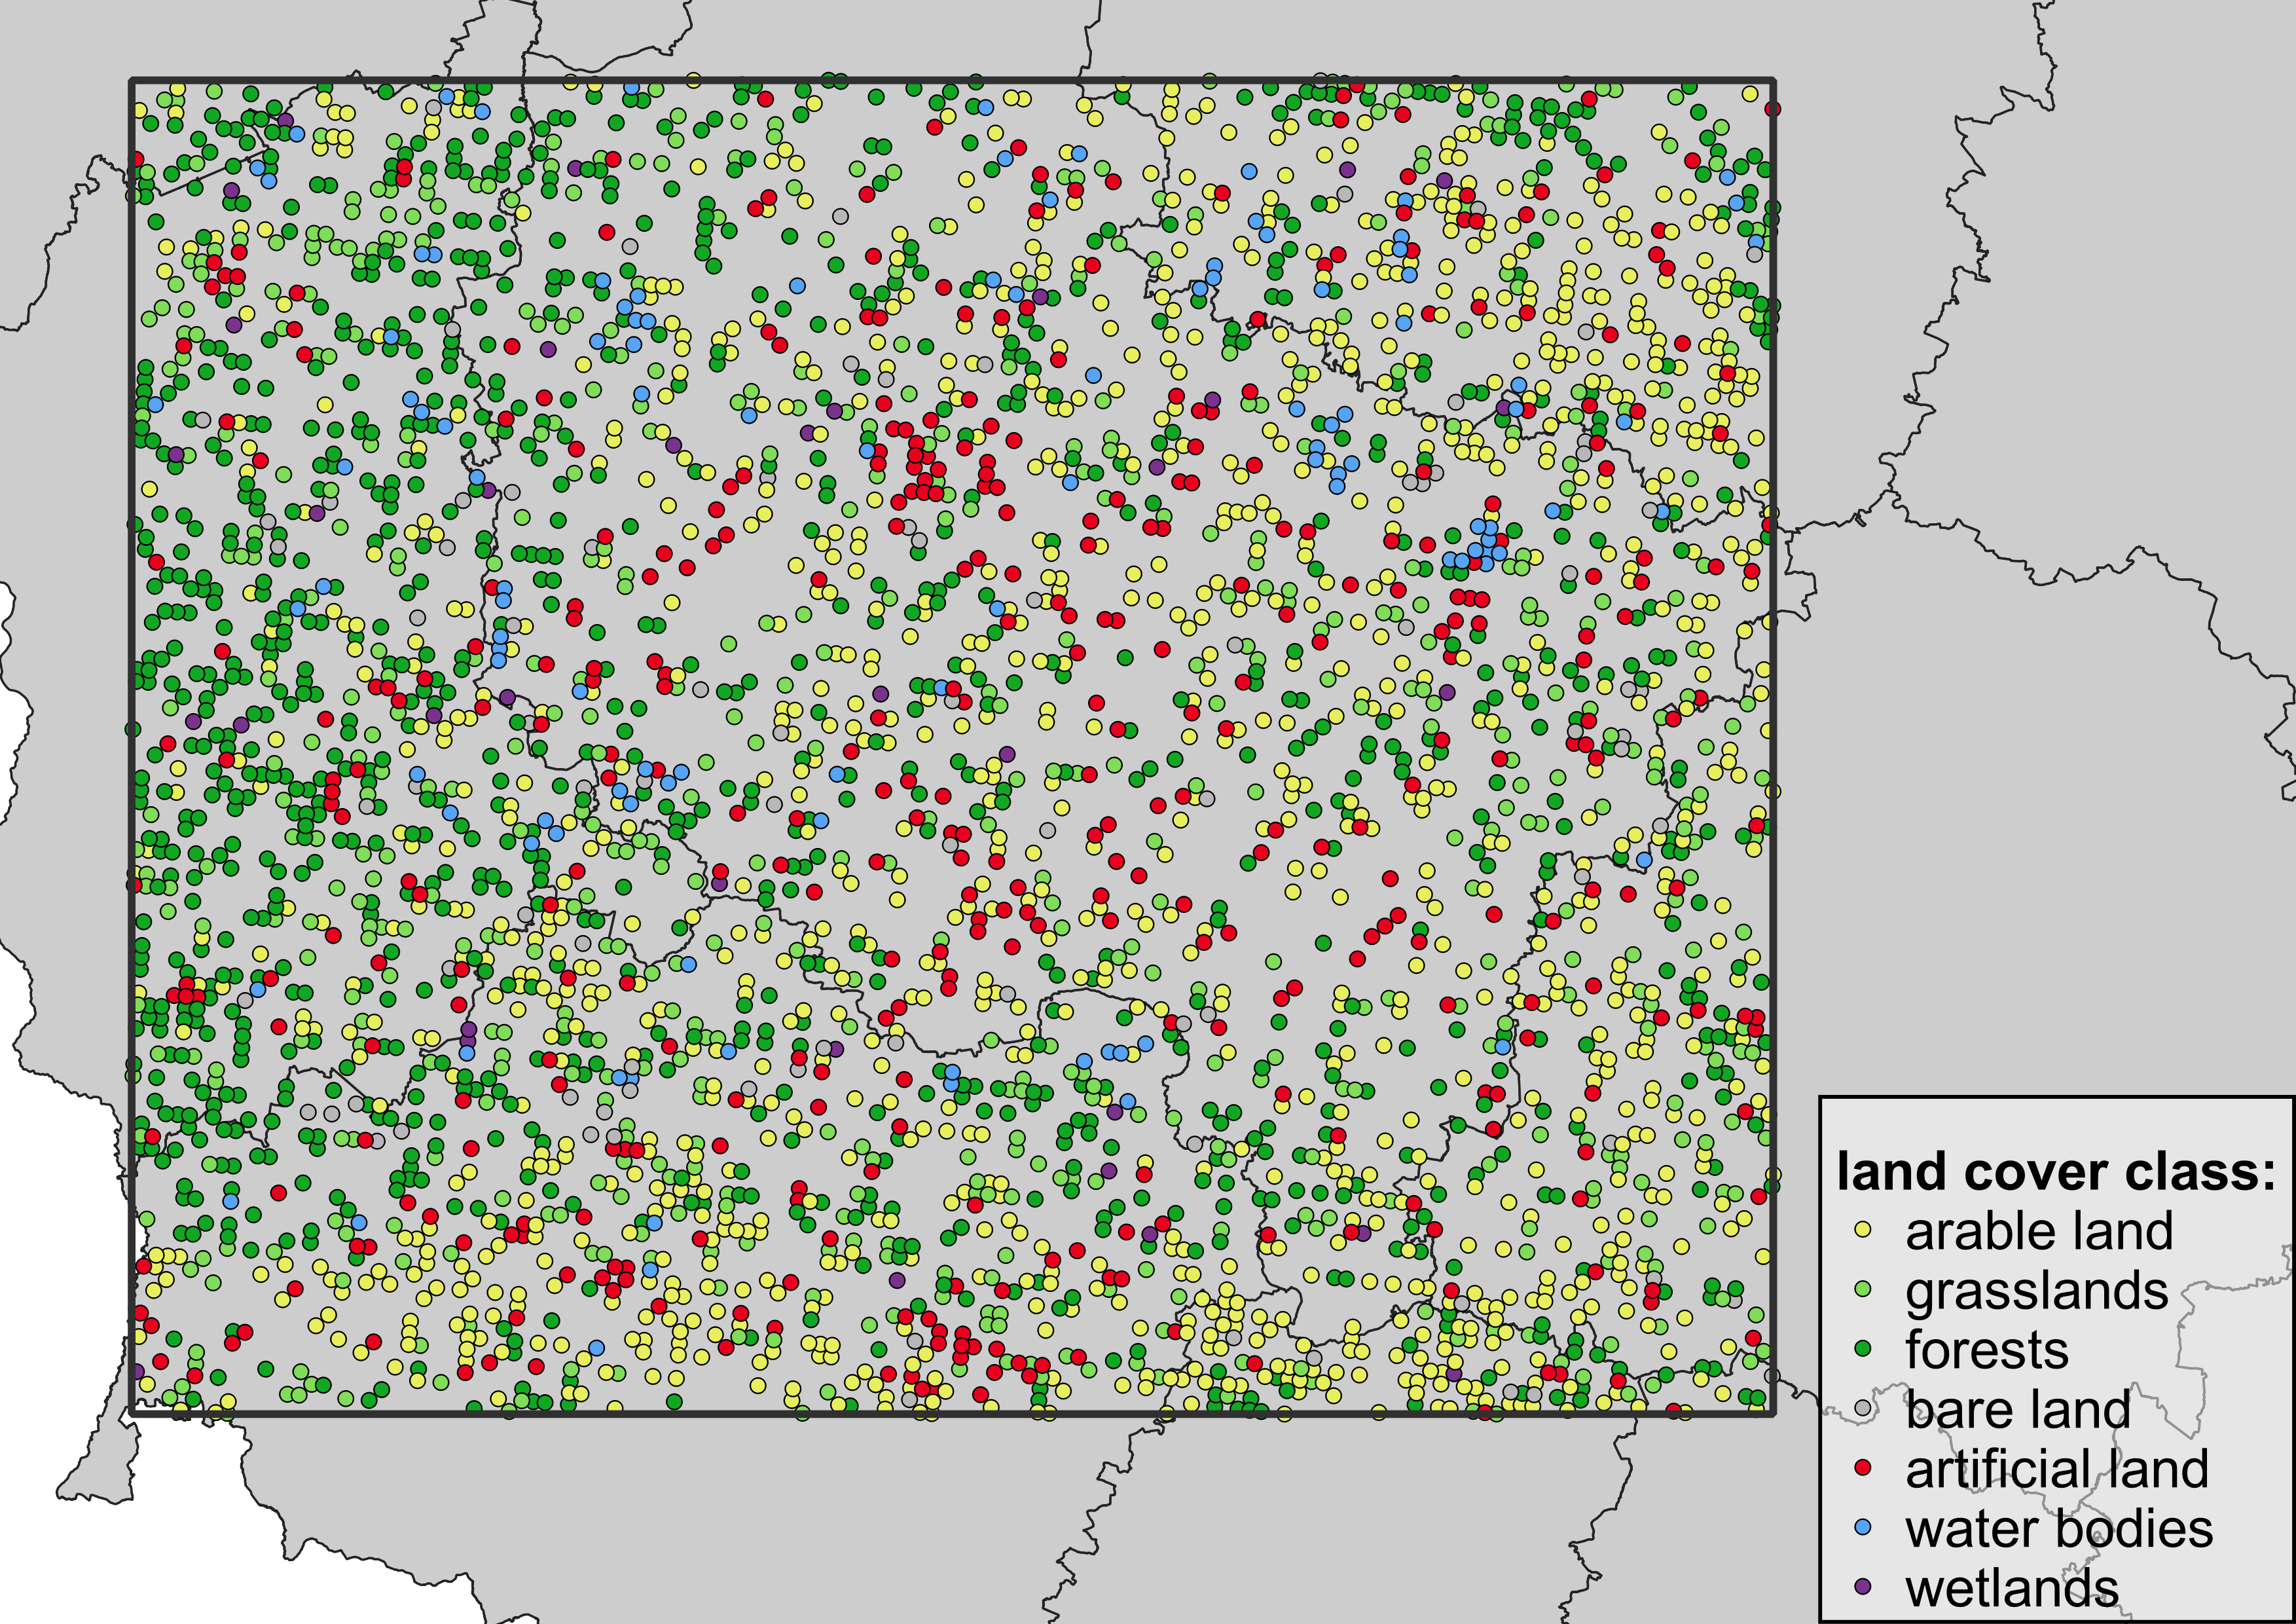
\includegraphics[width=1\textwidth,height=4.16667in]{./figures/lucas_distribution.png}

}

\caption{\label{fig-rycina3}Spatial distribution of LUCAS training
points after pre-processing}

\end{figure}

\hypertarget{sec-ml}{%
\section{Machine learning}\label{sec-ml}}

Machine learning is a computation method used to teach machines to learn
from datasets automatically without being specifically programmed
(\textcite{mahesh_machine_2018}; \textcite{sarker_machine_2021}). We can
divide machine learning methods into two main groups: supervised and
unsupervised.

Unsupervised learning analyzes unlabeled datasets without the need for
human intervention. This is widely used for extracting generative
features, identifying meaningful trends and structures, grouping results
and exploratory purposes \autocite{sarker_machine_2021}. This type of
machine learning discovers hidden patterns or data groupings (clusters)
which is used in exploratory analysis or objects segmentation. The most
common unsupervised learning algorithm is clustering. REF NEEDED

Supervised learning uses labeled training data and a collection of
training examples, which are used by an algorithm to find relationships
between different variables used to describe training data. It is
carried out when certain goals are identified to be accomplished from a
certain set of inputs. There are two types of supervised learning tasks:
classification (seperating data) and regression (fitting data)
\autocite{sarker_machine_2021}.

In this study, supervised classification algorithm called Random Forest
(RF) was used \autocite{breiman_random_2001}.

\hypertarget{sec-rf}{%
\subsection{Random forest algorithm}\label{sec-rf}}

I chose Random Forest as an algorithm used in this study. It is a very
popular machine learning tool thanks to its high interpretability and
relatively high accuracy \autocite{qi_random_2012}. Other advantages of
this algorithm is its ability to handle missing values, wide spectrum of
accepted variable types (continuous, binary, categorical) and ease of
modelling high-dimensional data \autocite{qi_random_2012}. Random Forest
consists of a specified number of decision trees, which are based on
series of splitting rules.

Decision tree aims to partition the dataset into smaller, more
homogeneous groups \autocite{kuhn_applied_2013}. This process creates a
set of rules by dividing dataset into several categories. Each rule in
the decision tree is specified by a feature (variable used to split) and
a threshold (value of a feature dividing dataset)
\autocite{sekulic_random_2020}. Random forest algorithm is characterized
by using many decision trees at the same time and receiving results by
applying majority voting system based on outputs of all decision trees
\autocite{kuhn_applied_2013}. Each tree in the forest has slightly
different input data - a subset of data is sampled with replacement to
get different result in every tree. This process is known as bagging or
bootstrap aggregating \autocite{schonlau_random_2020}.

\hypertarget{sec-tuning}{%
\subsection{Parameter tuning}\label{sec-tuning}}

Random Forest algorithm takes several hyper-parameters as an input in
order to specify how much should it fit to training data or how long
computation should take. Optimizing these parameters is crucial for
tree-based machine learning models \autocite{yang_hyperparameter_2020}.
Model's hyper-parameters can be fine-tuned to find values that give the
best model accuracy. I chose three hyper-parameters for tuning: number
of trees, maximum depth of the forest and minimal size of each node in
decision tree. Then, 10 models with different hyper-parameter values
chosen randomly from specified search space were created and trained. I
used overall accuracy achieved by each classifier to rank their
performance and choose parameters that best train the model. Parameters'
search spaces and tuning results can be found in Table
\ref{tbl-tabela3}.

\hypertarget{tbl-tabela3}{}
\begin{table}
\caption{\label{tbl-tabela3}Tuned parameters of RF model }\tabularnewline

\centering
\begin{tabular}{|>{}l|>{}l|>{}l|}
\toprule
\textbf{Hyper-parameter} & \textbf{Search space} & \textbf{Optimal value}\\
\midrule
number of trees & 50 - 400 & 272\\
\hline
maximum depth & 10 - 40 & 20\\
\hline
min. node size & 1 - 10 & 1\\
\bottomrule
\end{tabular}
\end{table}

\hypertarget{sec-resampling}{%
\subsection{Model quality assessment}\label{sec-resampling}}

Accuracy of the model was assessed with the help of four performance
measures:

\begin{itemize}
\item
  overall accuracy
\item
  Kappa coefficient
\item
  producer's accuracy
\item
  user's accuracy
\end{itemize}

SHORT DESCRIPTIONS OF MEASURES!!

I estimated values of these indices with the help of resampling
technique called spatial cross-validation (CV).

In \emph{n}-fold cross-validation, every data point is used in both
training and testing set. Whole dataset is randomly divided into
\emph{n} equal parts (\emph{folds}). Then, machine learning model is
independently trained \emph{n} times and in each run, different part of
the dataset is used as validation set while remaining \emph{n - 1} parts
are used to train the model. This way, every data point is used in
testing set only once but it is also used in training process
\autocite{jiao_performance_2016}. Usually, whole cross-validation
procedure is repeated several times to get higher number of unique
dataset splits and receive more reliable average values of the overall
accuracy \autocite{varga_validation_2021}. Such approach is a compromise
which enables possibility of using whole dataset in the training process
of the final model without a need of acquiring independent testing set.

Since this study is based on geographic data, Tobler's ``first law of
geography'' and spatial autocorrelation need to be taken into account.
Tobler stated that ``everything is related to everything else, but near
things are more related than distant things''. CITATION? In order to
prevent test points from being related to training points, I applied
spatial cross-validation approach which aims to prevent the model to
over-fit to the training data. This method is different than regular
cross-validation only in the partitioning step - instead of randomly
dividing dataset into groups, location of data points is used together
with k-means clustering \autocite{brenning_spatial_2012} in order to
create spatially disjoint folds \autocite{lovelace_geocomputation_2019}.
FIGURE? Thanks to this partitioning method, spatial-bias can be
significantly reduced which leads to more reliable performance
estimation.

With the aim to possibly accurately set values of model's
hyperparameters, I performed nested spatial cross-validation. This
method is an extension of previously described approach, but with tuning
added to the process. Each fold created in the spatial CV is further
divided into next \emph{k} folds which comprise the tuning level of the
process. Then, another cross-validation is performed on these folds in
order to determine performance of randomly sampled hyperparameter
values. The best of 10 hyperparameter combinations is chosen to train
the model on outer fold on performance estimation level
\autocite{schratz_hyperparameter_2019}. Whole process is then repeated
on every of \emph{n} outer folds which leads to most accurate
performance measurement as well as defining the best hyperparameter
setting. FIGURE?

\hypertarget{variable-importance-and-its-spatial-distribution}{%
\section{Variable importance and its spatial
distribution}\label{variable-importance-and-its-spatial-distribution}}

\begin{itemize}
\item
  calculating variable importance using DALEXtra package
\item
  calculating thermal band importance on aggregated raster
\item
  interpolating thermal band importance from training points
\end{itemize}

\hypertarget{sec-r}{%
\section{R language environment}\label{sec-r}}

Almost every step of analysis described in previous sections was
performed with use of R \autocite{R-base} - an open-source programming
language designed mainly for statistical computing and visualizing data.
I used RStudio \autocite{rstudio_team_rstudio_2020} as an integrated
development environment (IDE) created for R. Apart from base R
functionalities, I used a number of packages created by R community. We
used \emph{terra} package \autocite{R-terra} to perform raster data
operations and \emph{sf} \autocite{R-sf} to manipulate and process
vector data. To conduct machine learning steps of the analysis, we used
whole environment of various machine learning packages called
\emph{mlr3} \autocite{R-mlr3}. Random forest algorithm used by
\emph{mlr3} framework is part of \emph{ranger} package
\autocite{R-ranger} . I also used \emph{dplyr} \autocite{R-dplyr} and
\emph{tidyr} packages \autocite{R-tidyr} to clean and process tabular
data. \emph{DALEX} \autocite{R-DALEX} and \emph{DALEXtra}
\autocite{R-DALEXtra} packages provided various functionalities enabling
me to estimate variable importance and visualize these results with the
help of \emph{ggplot2} package \autocite{R-ggplot2}. Package called
\emph{gstat} \autocite{R-gstat} helped to interpolate variable
importance values from points to continuous raster layer. In addition,
\emph{future} package \autocite{R-future} was used to enable
multi-threading of some computationally intensive tasks.

\bookmarksetup{startatroot}

\hypertarget{sec-results-map}{%
\chapter{Result of the model - land cover map}\label{sec-results-map}}

\begin{itemize}
\item
  land cover map of Poznań metropolitan area
\item
  comparison of land cover map and RGB satellite imagery
\item
  probability map of model results
\end{itemize}

\begin{center}\rule{0.5\linewidth}{0.5pt}\end{center}

Część \textbf{Wyniki} może składać się z jednego lub więcej rozdziałów.
Każdy z tych rozdziałów powinien mieć tytuł adekwatny do swojej treści.

Rozdziały wynikowe powinny korzystać z wiedzy opisanej w poprzednich
rozdziałach (Rozdziały \textbf{?@sec-lit}, \textbf{?@sec-dane},
\textbf{?@sec-metody}). W przypadku prac analitycznych, ich treść
powinna przedstawiać kolejne etapy eksploracji i analizy danych. W
przypadku prac technicznych, treść tych rozdziałów powinna opisywać
stworzone narzędzia, a następnie pokazywać ich zastosowanie/a.

W przypadku prac technicznych warto pokazywać fragmenty napisanego
rozwiązania lub jego wywołania używając bloków kodu.

\begin{Shaded}
\begin{Highlighting}[]
\NormalTok{moja\_funkcja }\OtherTok{=} \ControlFlowTok{function}\NormalTok{(x)\{}
  \FunctionTok{cat}\NormalTok{(x, }\StringTok{"rządzi!"}\NormalTok{)}
\NormalTok{\}}
\FunctionTok{moja\_funkcja}\NormalTok{(}\StringTok{"Autor tej pracy"}\NormalTok{)}
\end{Highlighting}
\end{Shaded}

\begin{verbatim}
Autor tej pracy rządzi!
\end{verbatim}

\bookmarksetup{startatroot}

\hypertarget{sec-results-eval}{%
\chapter{Assessing model quality}\label{sec-results-eval}}

Table with quality indices:

\begin{itemize}
\item
  overall accuracy (OA) / classification error (CE)
\item
  producer's and user's accuracy (PA, UA)
\item
  Kappa coefficient
\end{itemize}

\begin{center}\rule{0.5\linewidth}{0.5pt}\end{center}

Część \textbf{Wyniki} może składać się z jednego lub więcej rozdziałów.
Każdy z tych rozdziałów powinien mieć tytuł adekwatny do swojej treści.

Rozdziały wynikowe powinny korzystać z wiedzy opisanej w poprzednich
rozdziałach (Rozdziały \textbf{?@sec-lit}, \textbf{?@sec-dane},
\textbf{?@sec-metody}). W przypadku prac analitycznych, ich treść
powinna przedstawiać kolejne etapy eksploracji i analizy danych. W
przypadku prac technicznych, treść tych rozdziałów powinna opisywać
stworzone narzędzia, a następnie pokazywać ich zastosowanie/a.

W przypadku prac technicznych warto pokazywać fragmenty napisanego
rozwiązania lub jego wywołania używając bloków kodu.

\begin{Shaded}
\begin{Highlighting}[]
\NormalTok{moja\_funkcja }\OtherTok{=} \ControlFlowTok{function}\NormalTok{(x)\{}
  \FunctionTok{cat}\NormalTok{(x, }\StringTok{"rządzi!"}\NormalTok{)}
\NormalTok{\}}
\FunctionTok{moja\_funkcja}\NormalTok{(}\StringTok{"Autor tej pracy"}\NormalTok{)}
\end{Highlighting}
\end{Shaded}

\begin{verbatim}
Autor tej pracy rządzi!
\end{verbatim}

\bookmarksetup{startatroot}

\hypertarget{sec-results-therm}{%
\chapter{Evaluation of thermal band's impact on prediction
results}\label{sec-results-therm}}

\hypertarget{sec-imp-overall}{%
\section{Overall importance of thermal band}\label{sec-imp-overall}}

\begin{itemize}
\item
  mean temperature for every predicted land cover class
\item
  variable importance plots, variable profiles
\item
  mean importance of thermal band on each land cover class
\end{itemize}

\hypertarget{sec-imp-spat}{%
\section{Spatial distribution of thermal band's
importance}\label{sec-imp-spat}}

\begin{itemize}
\item
  thermal band importance map (two methods: raster aggregation and
  interpolation of importance in LUCAS points)
\item
  difference raster map between prediction with and without thermal band
  included, transition matrix
\end{itemize}

\begin{center}\rule{0.5\linewidth}{0.5pt}\end{center}

Część \textbf{Wyniki} może składać się z jednego lub więcej rozdziałów.
Każdy z tych rozdziałów powinien mieć tytuł adekwatny do swojej treści.

Rozdziały wynikowe powinny korzystać z wiedzy opisanej w poprzednich
rozdziałach (Rozdziały \textbf{?@sec-lit}, \textbf{?@sec-dane},
\textbf{?@sec-metody}). W przypadku prac analitycznych, ich treść
powinna przedstawiać kolejne etapy eksploracji i analizy danych. W
przypadku prac technicznych, treść tych rozdziałów powinna opisywać
stworzone narzędzia, a następnie pokazywać ich zastosowanie/a.

W przypadku prac technicznych warto pokazywać fragmenty napisanego
rozwiązania lub jego wywołania używając bloków kodu.

\begin{Shaded}
\begin{Highlighting}[]
\NormalTok{moja\_funkcja }\OtherTok{=} \ControlFlowTok{function}\NormalTok{(x)\{}
  \FunctionTok{cat}\NormalTok{(x, }\StringTok{"rządzi!"}\NormalTok{)}
\NormalTok{\}}
\FunctionTok{moja\_funkcja}\NormalTok{(}\StringTok{"Autor tej pracy"}\NormalTok{)}
\end{Highlighting}
\end{Shaded}

\begin{verbatim}
Autor tej pracy rządzi!
\end{verbatim}

\bookmarksetup{startatroot}

\hypertarget{conclusion}{%
\chapter{Conclusion}\label{conclusion}}

\begin{itemize}
\item
  land cover map of Poznań metropolitan area was created, impact of
  thermal band on classification results was measured
\item
  despite thermal band having low overall impact on model results, there
  is a strong spatial auto-correlation for its importance
\item
  land surface temperature was especially significant for land cover
  classification of urban areas, it helped in identify built-up areas
\item
  it may mean that thermal band will become increasingly important in
  studies on urban sprawl and suburbanisation
\item
  better land cover maps will help in better management of metropolitan
  areas growth and quantifying impact of urbanisation on natural
  environment more precisely
\end{itemize}

\begin{center}\rule{0.5\linewidth}{0.5pt}\end{center}

Podsumowanie pracy jest w pewnym sensie znacznie rozbudowanym
abstraktem. Należy wyliczyć i opisać osiągnięcia uzyskane w pracy
dyplomowej. Tutaj jednak (w przeciwieństwie do np. rozdziału
\textbf{?@sec-wprowadzenie}) należy przechodzić od szczegółu do ogółu -
co zostało stworzone/określone, jak zostało to zrobione, jakie ma to
konsekwencje, itd.

Ten rozdział powinien też zawierać opis kwestii, których nie udało się
rozwiązać w pracy dyplomowej (i dlaczego się nie udało) oraz pomysły na
przyszłe ulepszenie uzyskanych wyników lub dalsze badania.

\printbibliography[heading=bibintoc, title=Bibliography]

\end{document}
